\documentclass[aspectratio=169]{beamer}
\usetheme{Madrid}
\usecolortheme{default}

\usepackage{fontspec}
\usepackage{polyglossia}
\setmainlanguage{english}
\usepackage{graphicx}
\usepackage{amsmath}
\usepackage{booktabs}
\usepackage{xcolor}

\definecolor{examplecolor}{RGB}{180,83,9}

\setbeamertemplate{navigation symbols}{}
\setbeamertemplate{footline}[frame number]
\setbeamerfont{footnote}{size=\tiny}

\newcommand{\fuente}[1]{{\footnotesize\textit{Source: #1}}}
\newcommand{\ejemplo}[1]{\par\vspace{0.4em}{\small\color{examplecolor}\textbf{Example:} #1}}

\title[3. Unsupervised Learning]{Chapter 3: Unsupervised\\Learning}
\subtitle{Course material}
\author{Universidad de Salamanca}
\institute{Faculties of Sciences and Chemical Sciences}
\date{\today}

\begin{document}

% ============================================================
\begin{frame}
  \titlepage
\end{frame}

\begin{frame}{In this chapter}
  \begin{enumerate}
    \item \textbf{3.1 Clustering}: grouping data without labels
    \item \textbf{3.2 Dimensionality reduction}: simplifying and visualizing complex data
    \item \textbf{3.3 Anomaly detection}: identifying rare or suspicious cases
  \end{enumerate}
\end{frame}

\begin{frame}{What is unsupervised learning?}
  \begin{itemize}
    \item There are no labels: we only have input data $X$, no correct answers $y$
    \item The system must discover the \textbf{latent structure} of the data on its own
    \item Yann LeCun's quote: \textit{``If intelligence is a cake, unsupervised learning is the cake, supervised learning is the icing, and reinforcement learning is the cherry''}
  \end{itemize}
  \ejemplo{the vast majority of real-world data is unlabeled: photos, text, transactions... that's why this paradigm matters so much in practice.}
\end{frame}

\begin{frame}{Practical applications}
  \begin{itemize}
    \item \textbf{Market segmentation}: grouping customers into homogeneous niches without defining the categories in advance
    \item \textbf{Visualization}: projecting data with hundreds of variables into 2D or 3D to understand it at a glance
    \item \textbf{Recommendation systems}: grouping users or products with similar tastes
    \item \textbf{Anomaly detection}: spotting fraud or manufacturing defects never seen before
  \end{itemize}
\end{frame}

% ============================================================
\section{3.1 Clustering}

\begin{frame}{What is clustering?}
  \begin{itemize}
    \item Goal: split the data into subgroups with \textbf{high internal similarity} and \textbf{high external differentiation}
    \item There's no ``ground truth'': the system must discover the structure on its own
    \item Main algorithms: $K$-means, hierarchical, DBSCAN
  \end{itemize}
\end{frame}

\begin{frame}{$K$-means: the algorithm's cycle}
  \footnotesize
  \begin{enumerate}
    \item \textbf{Initialization}: $K$ centroids are chosen
    \item \textbf{Assignment}: each sample joins its nearest centroid
    \item \textbf{Update}: each centroid is recomputed as the mean of its group
    \item Repeat until the centroids stop moving (\textbf{convergence})
  \end{enumerate}
  \begin{center}
    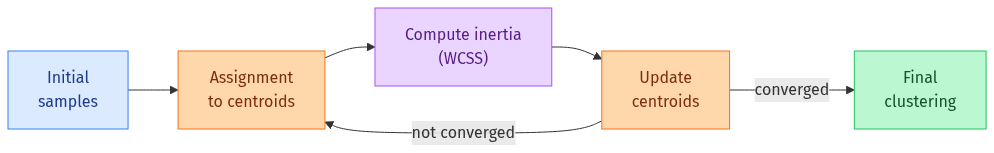
\includegraphics[width=0.62\textwidth]{../book/_static/generated/diagrams_pdf/en/02_unsupervised_learning_01_clustering_01.png}
  \end{center}
\end{frame}

\begin{frame}{$K$-means: the process, visually}
  \begin{center}
    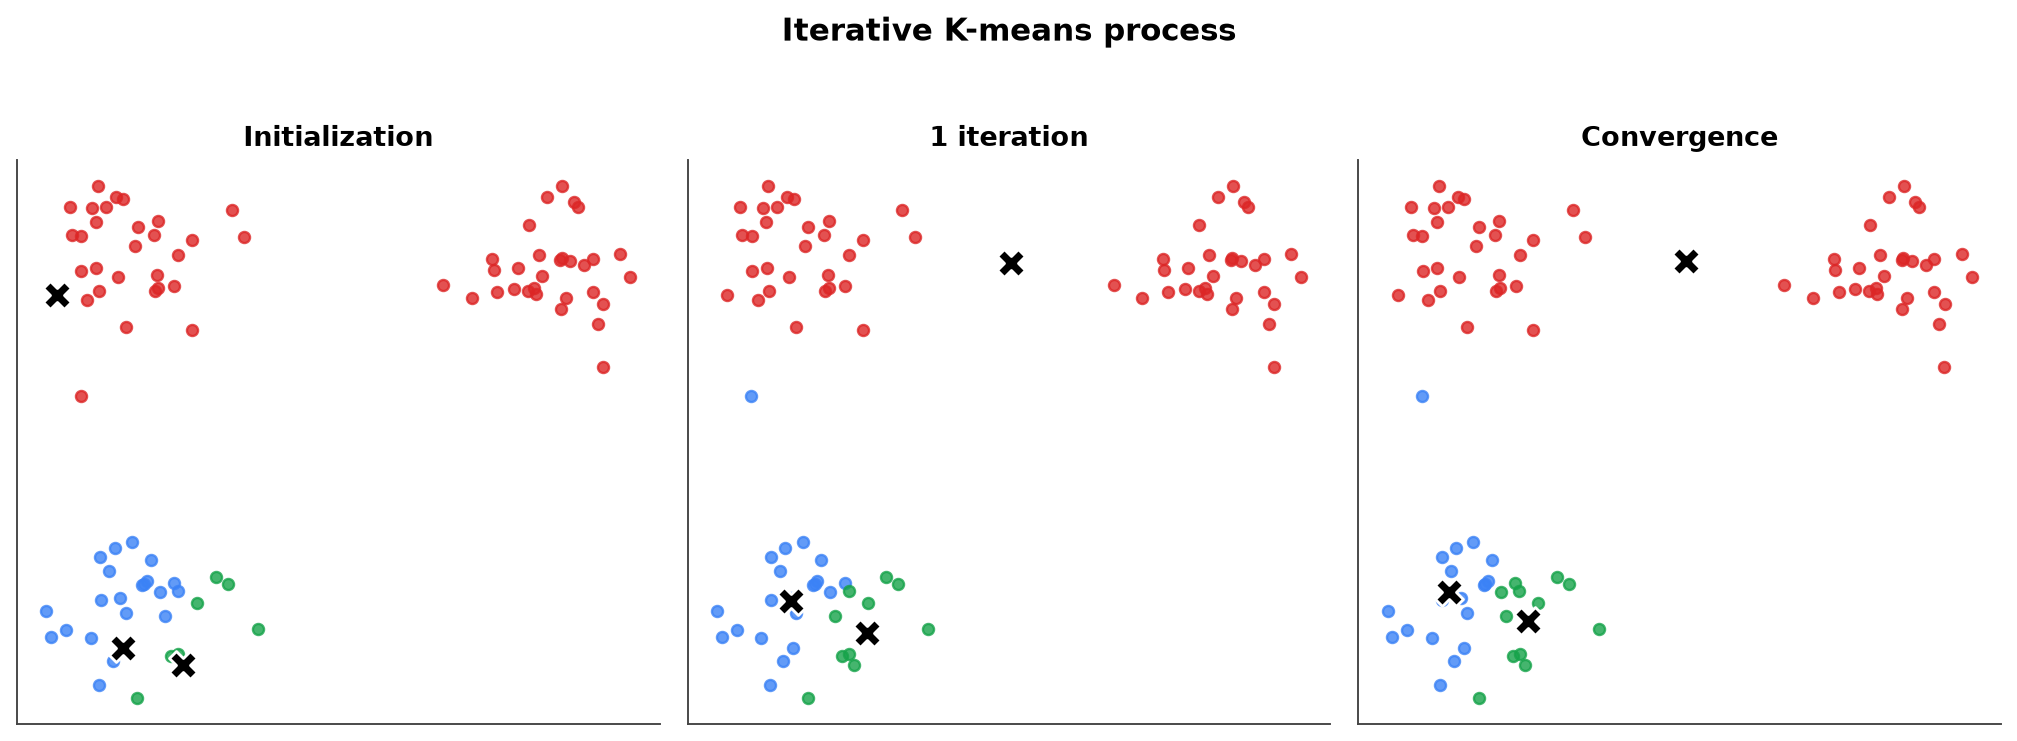
\includegraphics[width=0.85\textwidth]{../book/_static/generated/figures/en/kmeans_process.png}
  \end{center}
  \ejemplo{it's like seating guests at a party: each guest sits at the nearest table, then each table recenters on its guests, and this repeats until no one moves.}
\end{frame}

\begin{frame}{$K$-means++ and the elbow method}
  \begin{itemize}
    \item $K$-means is sensitive to initialization: poorly placed centroids can lead to a suboptimal result
    \item \textbf{$K$-means++}: picks initial centroids as far apart as possible, speeding up convergence
    \item How many groups $K$ to choose? The \textbf{elbow method}: find the point where inertia stops dropping sharply
  \end{itemize}
  \begin{center}
    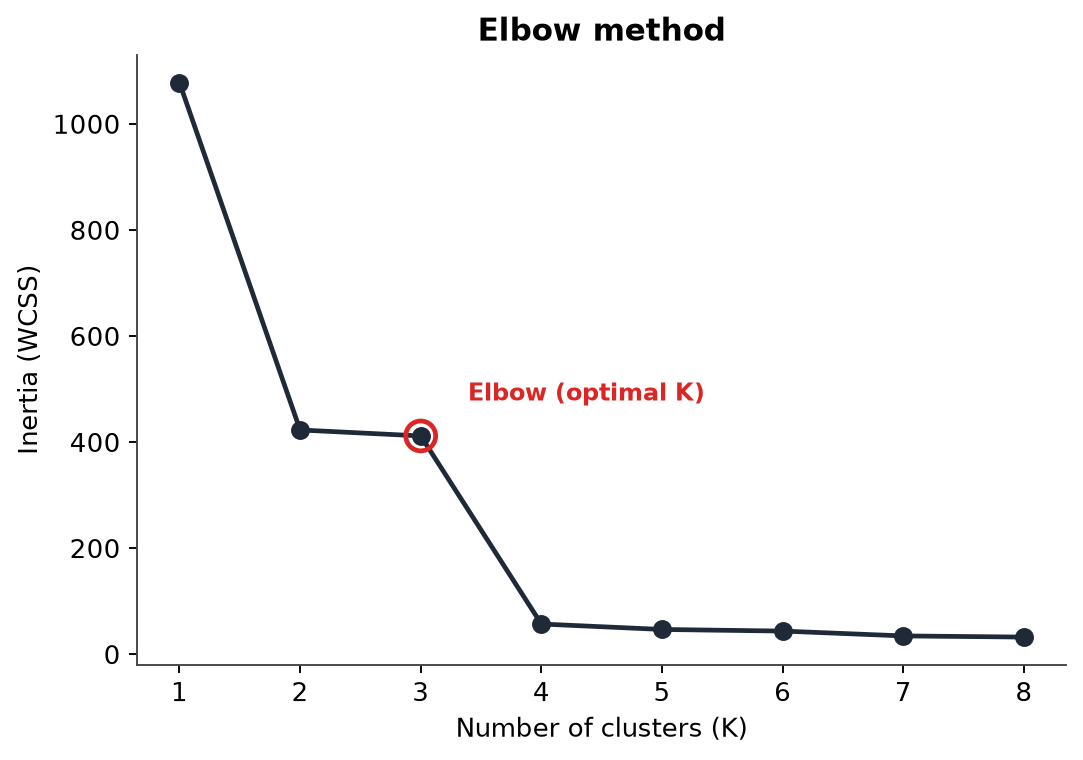
\includegraphics[width=0.42\textwidth]{../book/_static/generated/figures/en/elbow_method.png}
  \end{center}
\end{frame}

\begin{frame}{Hierarchical clustering}
  \begin{itemize}
    \item Doesn't require fixing $K$ in advance
    \item \textbf{Agglomerative} approach (bottom-up): each point starts as its own group, and at each step the two closest groups merge
    \item The result is visualized as a \textbf{dendrogram}; cutting it at a given height determines the final number of groups
  \end{itemize}
  \begin{center}
    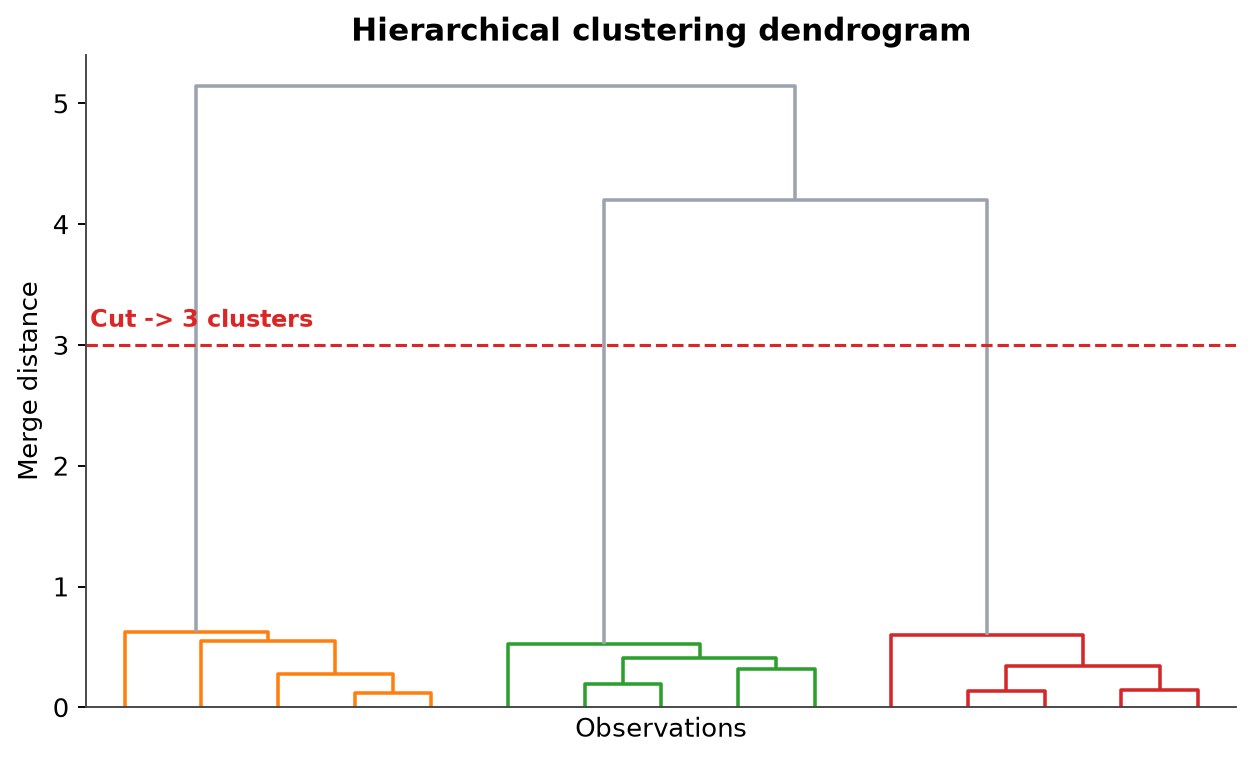
\includegraphics[width=0.52\textwidth]{../book/_static/generated/figures/en/dendrogram.png}
  \end{center}
\end{frame}

\begin{frame}{Linkage criteria}
  \begin{itemize}
    \item Define how to measure distance between two groups, not between two points
    \item \textbf{Complete}: \textit{maximum} distance between members --- compact, balanced groups
    \item \textbf{Single}: \textit{minimum} distance --- sensitive to noise, tends to chain elongated groups
    \item \textbf{Average}: mean of all distances --- a balance between the two above
  \end{itemize}
  \begin{center}
    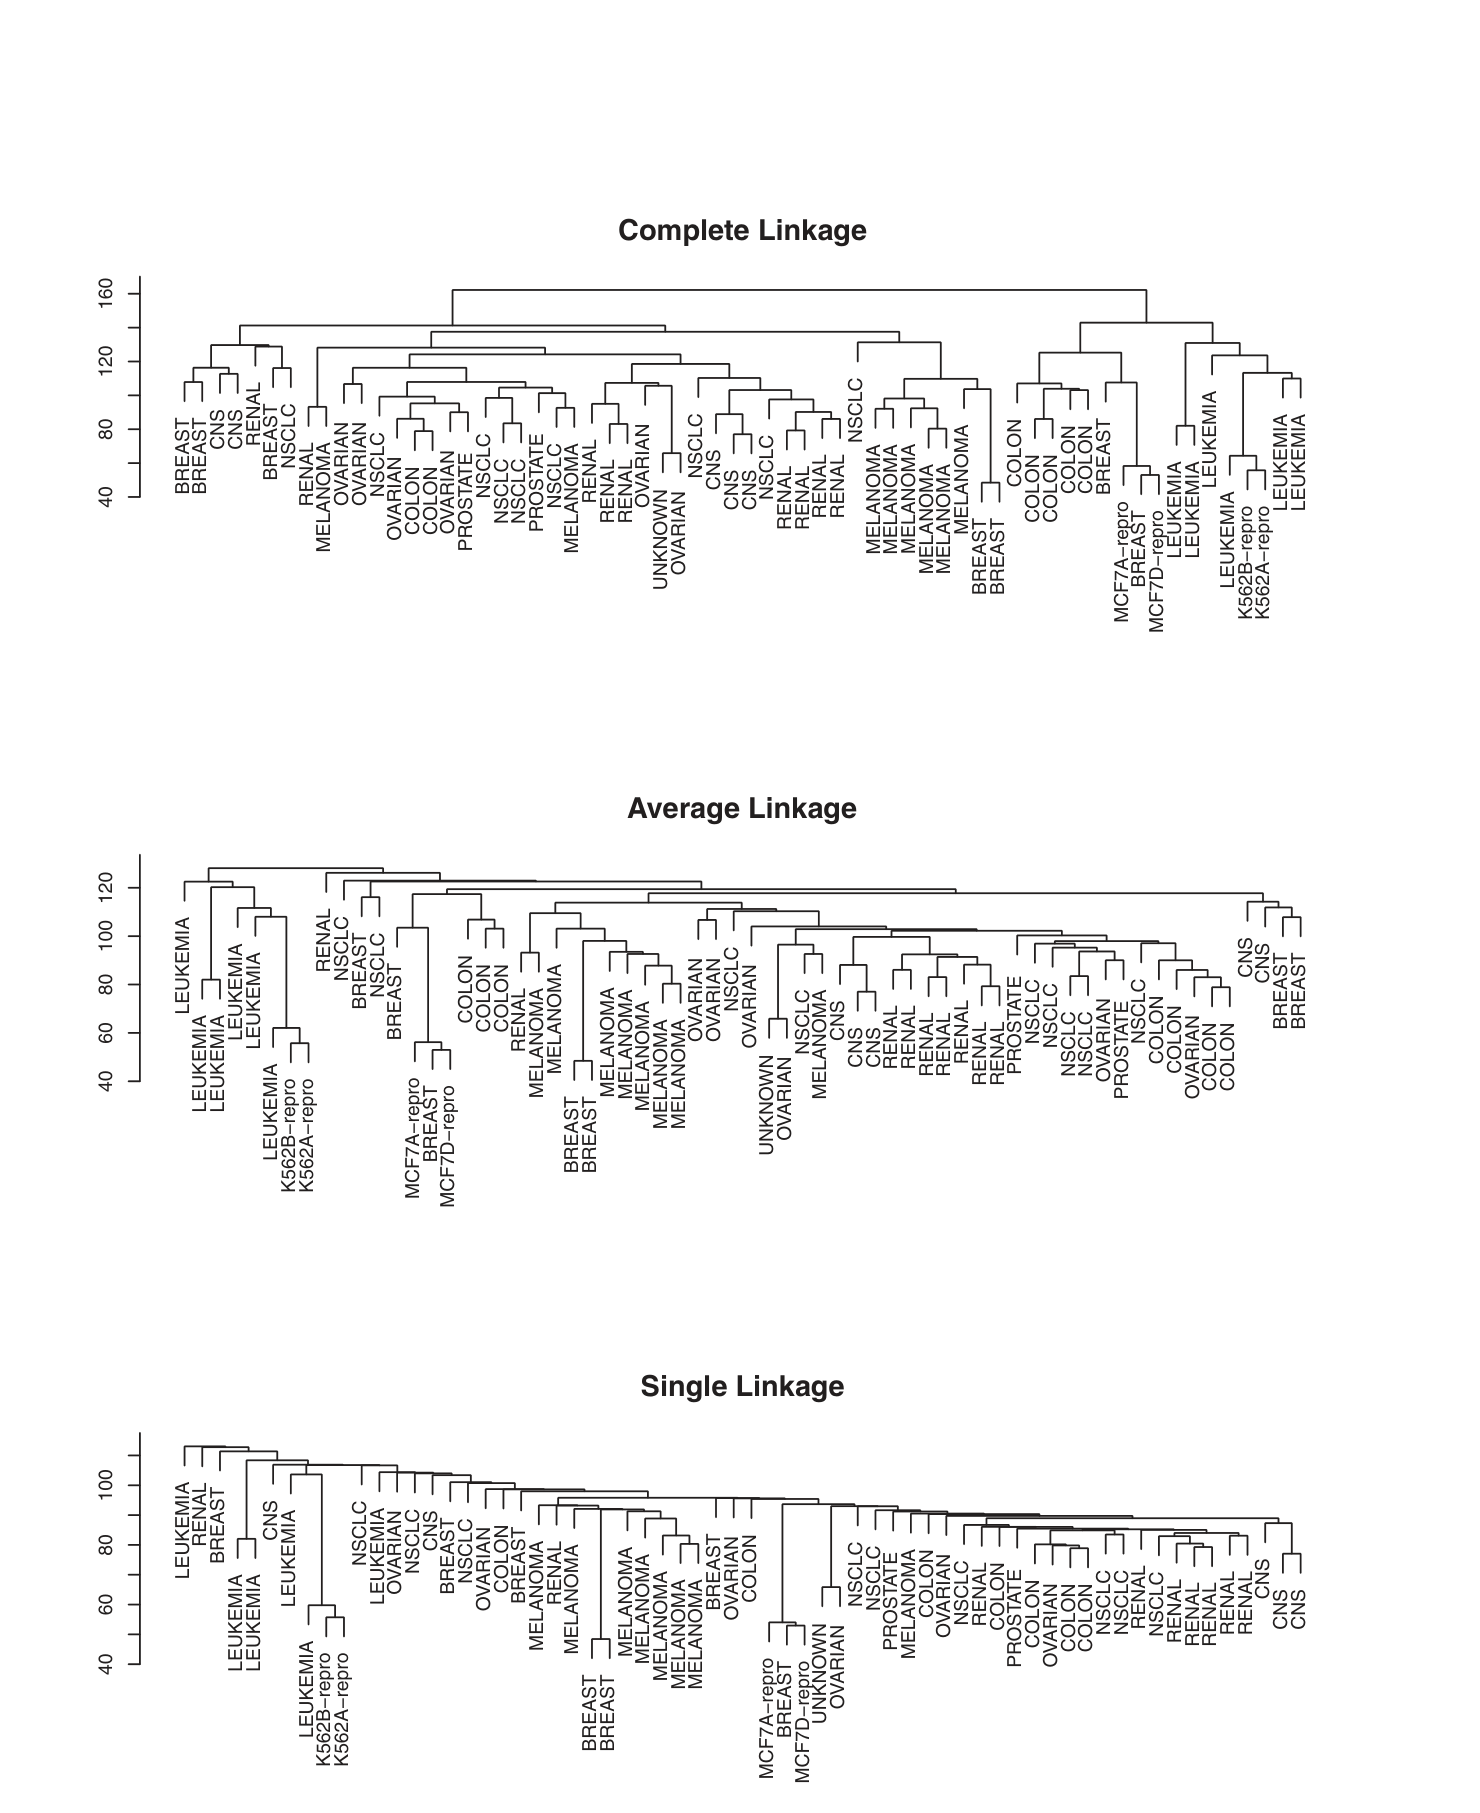
\includegraphics[width=0.26\textwidth]{../book/_static/book_figures/islr_fig10_17_nci60_dendrogram.png}
  \end{center}
  \fuente{James, Witten, Hastie \& Tibshirani (2013), \textit{An Introduction to Statistical Learning}, Fig. 10.17.}
\end{frame}

\begin{frame}{DBSCAN: density-based clustering}
  \begin{itemize}
    \item Defines groups by \textbf{local density}, not by closeness to a centroid
    \item Two parameters: \textbf{$\epsilon$} (neighborhood radius) and \textbf{MinPts} (minimum neighbors to be dense)
    \item Three point types: \textbf{core} (dense), \textbf{border} (near a core point), and \textbf{noise} (isolated)
  \end{itemize}
  \begin{center}
    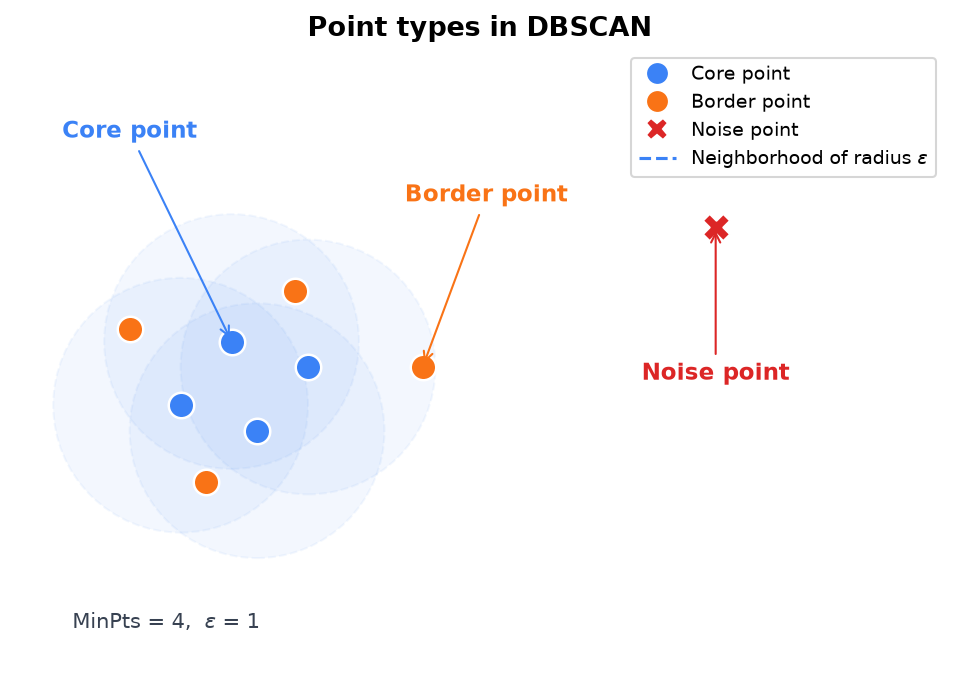
\includegraphics[width=0.45\textwidth]{../book/_static/generated/figures/en/dbscan_point_types.png}
  \end{center}
\end{frame}

\begin{frame}{DBSCAN vs. $K$-means}
  \begin{itemize}
    \item DBSCAN detects \textbf{arbitrary shapes} (not just spherical) and isolates noise natively
    \item $K$-means forces every point into a group, even outliers
  \end{itemize}
  \begin{center}
    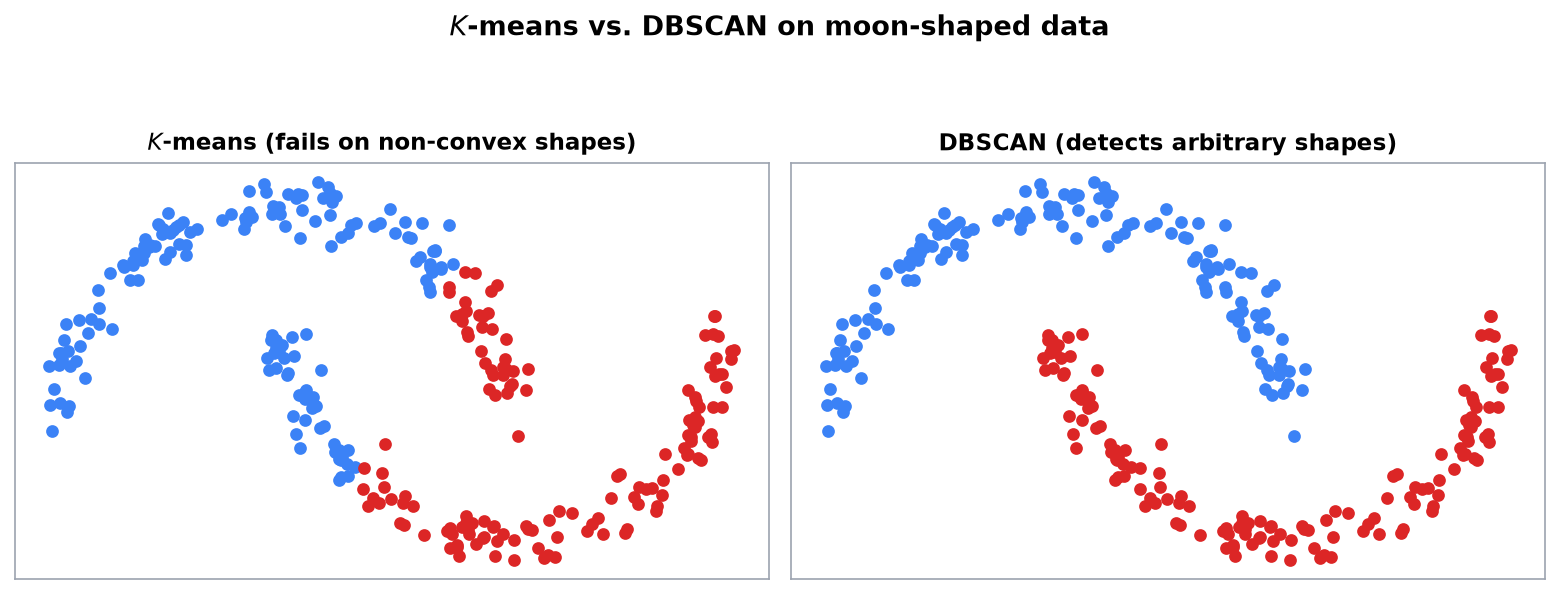
\includegraphics[width=0.72\textwidth]{../book/_static/generated/figures/en/dbscan_vs_kmeans.png}
  \end{center}
\end{frame}

\begin{frame}{Evaluation: silhouette coefficient}
  \begin{itemize}
    \item Without labels, how do we know if a clustering is good?
    \item The silhouette coefficient compares, for each point, its \textbf{cohesion} (distance to its own group) with its \textbf{separation} (distance to the nearest other group)
    \item Range $[-1, 1]$: near $+1$ is a good grouping; near $0$, an ambiguous boundary; negative, likely misassigned
    \item Other criteria exist (AIC/BIC, purity, Rand index...) to compare against already-known labels
  \end{itemize}
  \begin{center}
    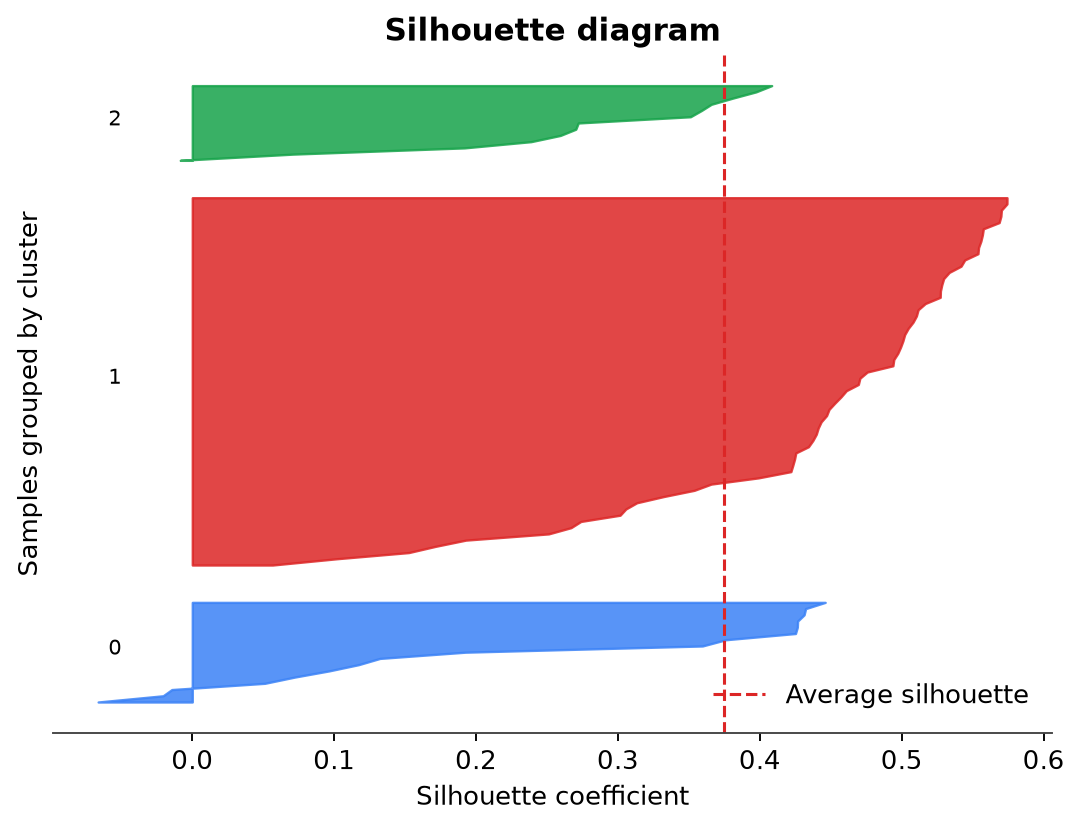
\includegraphics[width=0.3\textwidth]{../book/_static/generated/figures/en/silhouette_diagram.png}
  \end{center}
\end{frame}

\begin{frame}{Summary: 3.1 Clustering}
  \begin{itemize}
    \item \textbf{$K$-means}: simple and fast, but needs a known $K$ and roughly spherical groups
    \item \textbf{Hierarchical}: no $K$ needed, gives a visual, interpretable dendrogram
    \item \textbf{DBSCAN}: detects arbitrary shapes and isolates noise automatically
    \item \textbf{Silhouette}: standard metric to evaluate quality without labels
  \end{itemize}
\end{frame}

% ============================================================
\section{3.2 Dimensionality reduction}

\begin{frame}{The curse of dimensionality}
  \begin{itemize}
    \item As dimensions increase, the space becomes \textbf{ultra-sparse}
    \item Samples tend to sit at the boundary of the space, not in the center
    \item Distances between points become nearly indistinguishable, degrading distance-based algorithms (like $K$-NN)
  \end{itemize}
  \begin{center}
    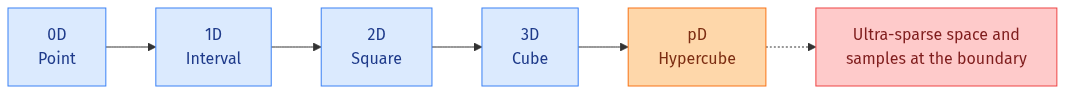
\includegraphics[width=0.85\textwidth]{../book/_static/generated/diagrams_pdf/en/02_unsupervised_learning_02_dimensionality_reduction_01.png}
  \end{center}
\end{frame}

\begin{frame}{Why reduce dimensions?}
  \begin{itemize}
    \item Drastically speeds up computation
    \item Mitigates overfitting
    \item Indispensable for \textbf{visualizing} complex data in 2D or 3D
  \end{itemize}
  \begin{center}
    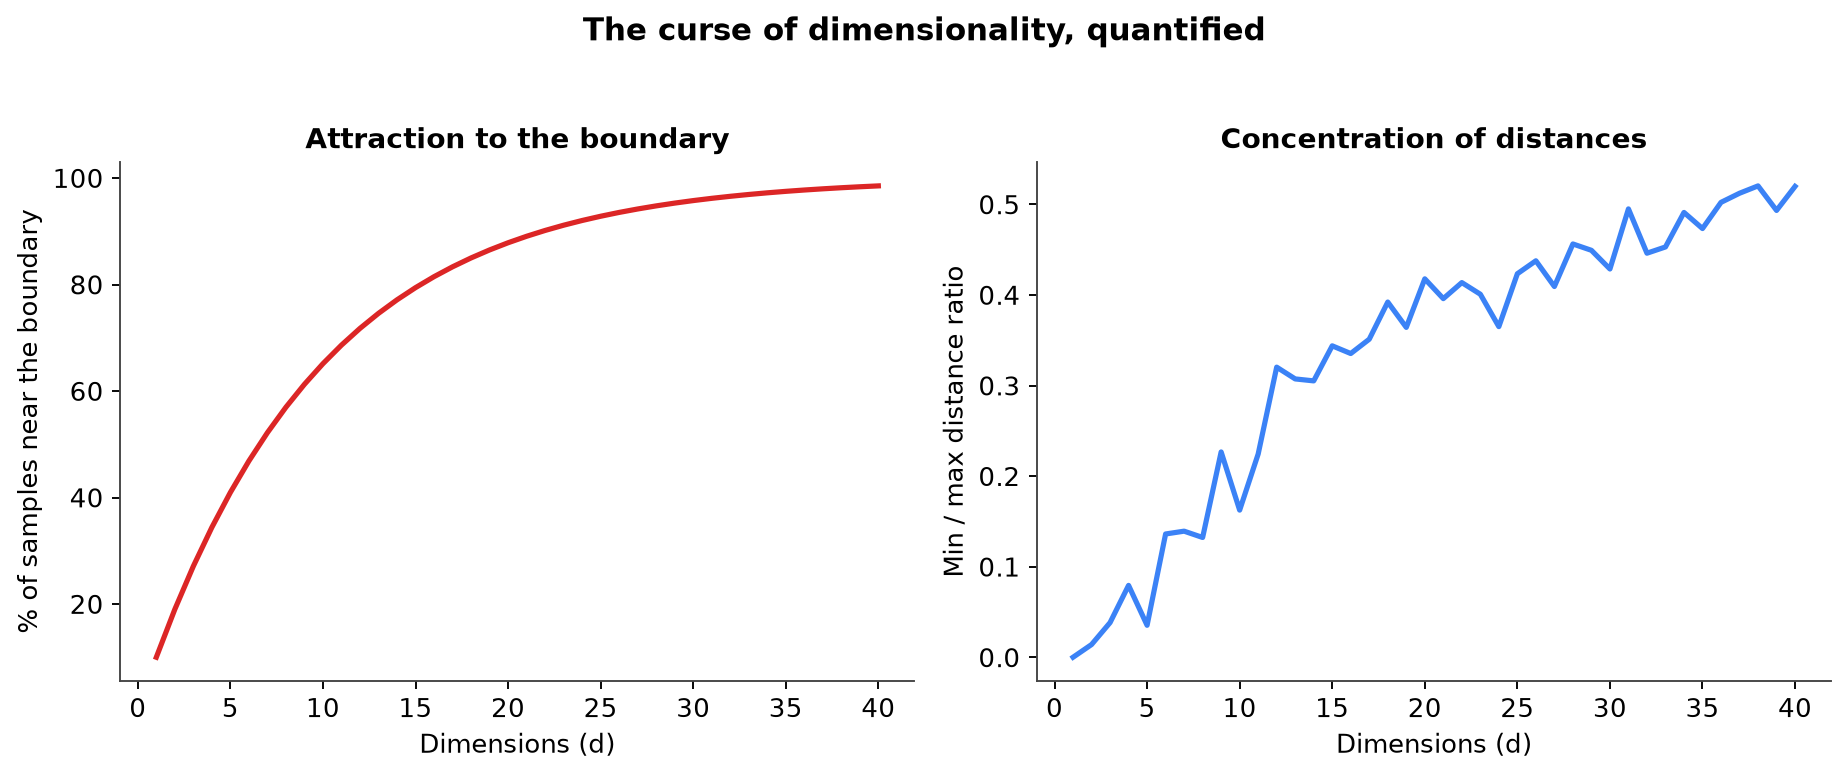
\includegraphics[width=0.85\textwidth]{../book/_static/generated/figures/en/curse_of_dimensionality.png}
  \end{center}
\end{frame}

\begin{frame}{PCA: the direction of maximum variance}
  \begin{itemize}
    \item PCA projects the data onto the axes where it \textbf{varies most}, losing as little information as possible
    \item PC1: the direction of maximum variance; PC2: orthogonal to PC1, captures the remaining variance
  \end{itemize}
  \begin{center}
    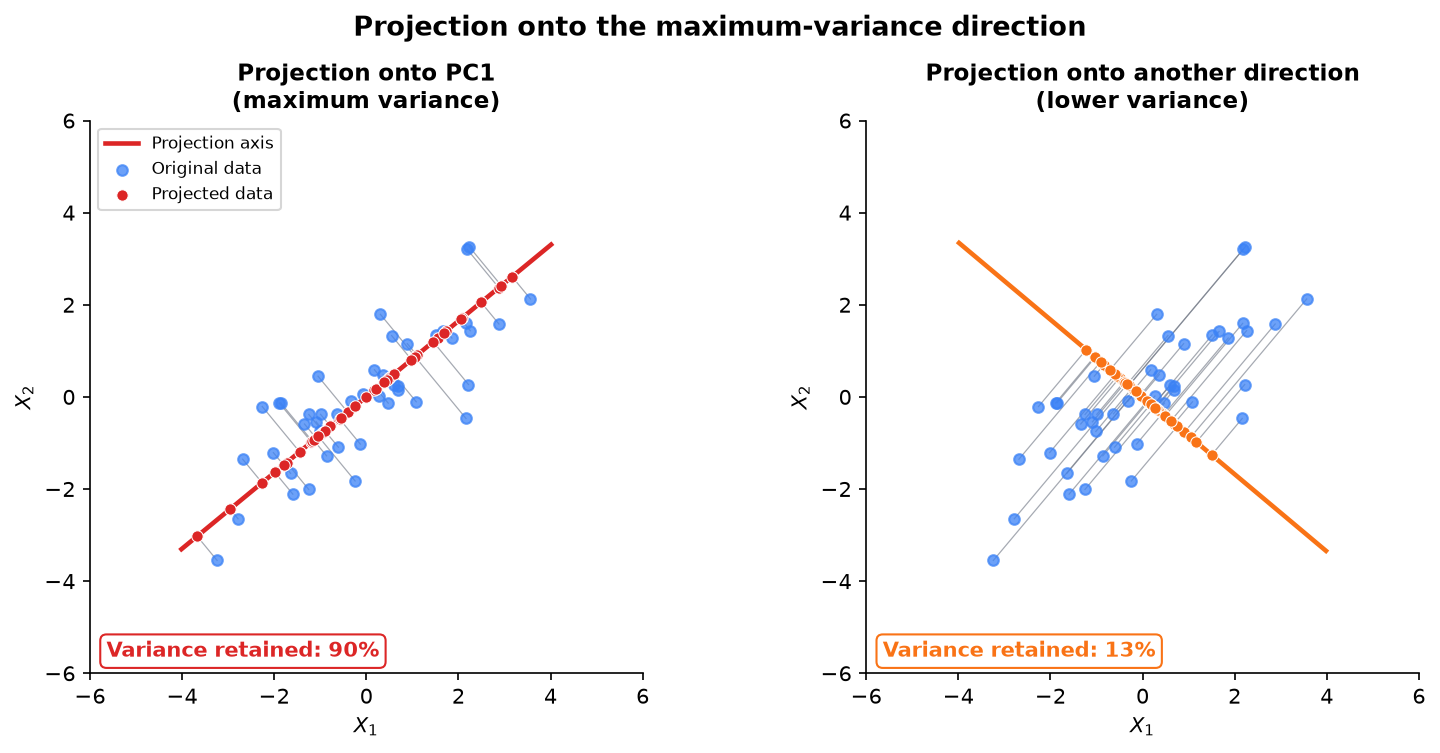
\includegraphics[width=0.68\textwidth]{../book/_static/generated/figures/en/pca_max_variance_projection.png}
  \end{center}
\end{frame}

\begin{frame}{PCA: principal components}
  \begin{itemize}
    \item Computed via singular value decomposition (SVD) of the data matrix
    \item Can be seen as a \textbf{linear autoencoder}: compress then reconstruct, minimizing the error
  \end{itemize}
  \begin{center}
    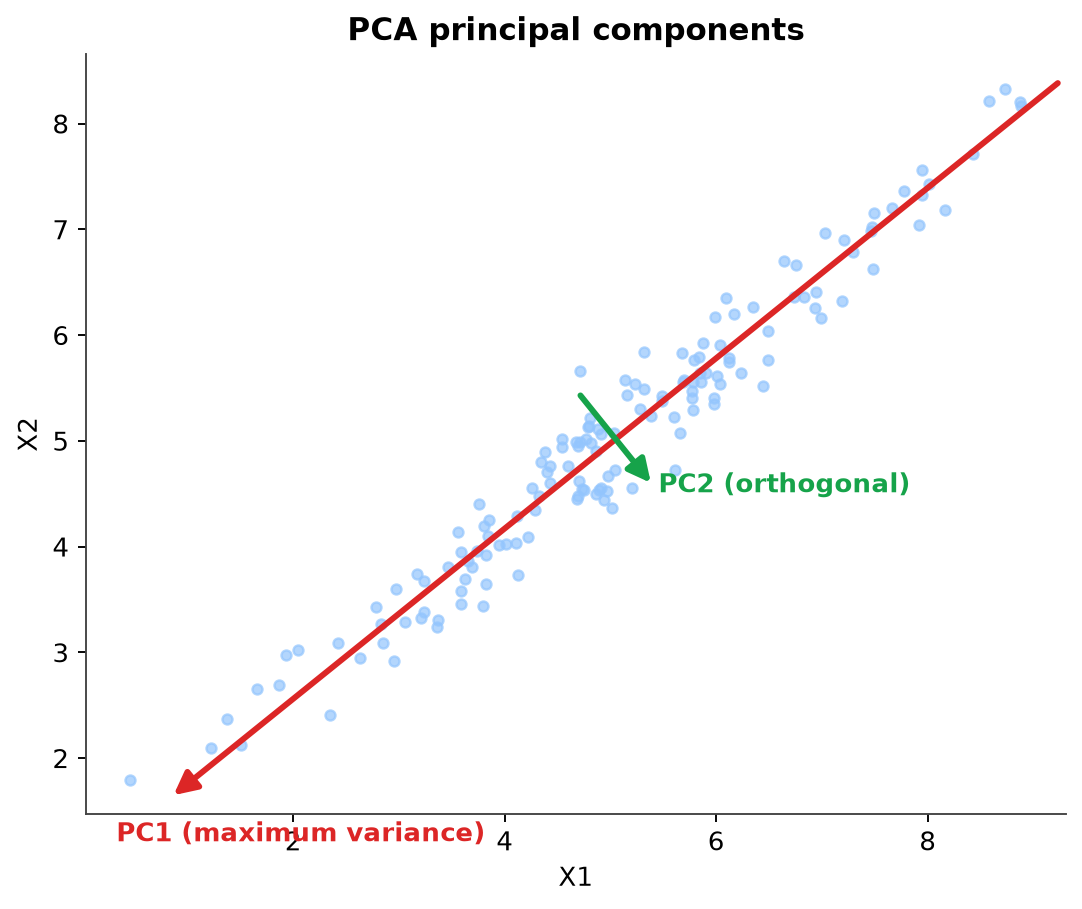
\includegraphics[width=0.4\textwidth]{../book/_static/generated/figures/en/pca_projection.png}
  \end{center}
\end{frame}

\begin{frame}{PCA on real data: NCI60 (6830 genes)}
  \footnotesize
  From 6830 genes down to just 3 principal components: lines of the same cancer type (same color) cluster together despite the huge original dimensionality.
  \begin{center}
    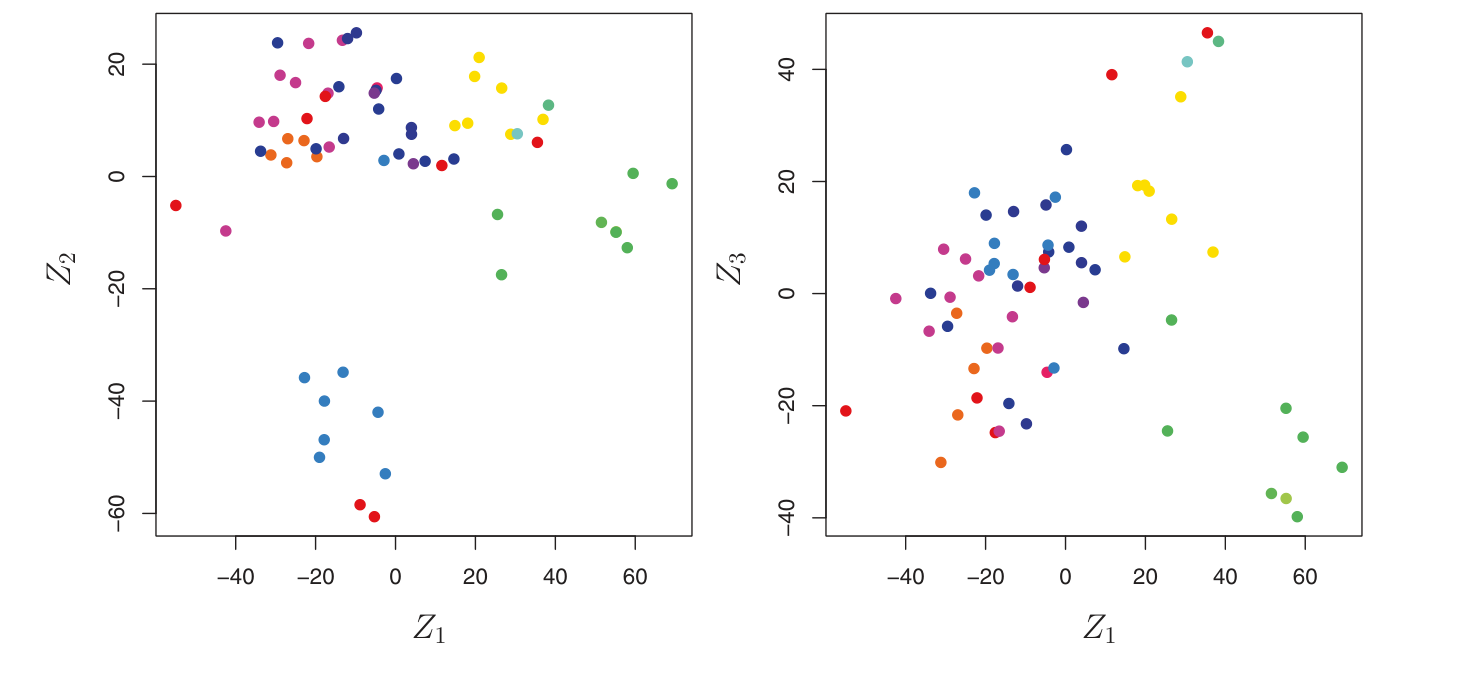
\includegraphics[width=0.62\textwidth]{../book/_static/book_figures/islr_fig10_15_nci60_pca.png}
  \end{center}
  \fuente{James, Witten, Hastie \& Tibshirani (2013), \textit{An Introduction to Statistical Learning}, Fig. 10.15.}
\end{frame}

\begin{frame}{Manifold learning: when data isn't flat}
  \begin{itemize}
    \item PCA assumes the interesting structure is \textbf{linear} --- it fails on curved structures
    \item The \textbf{manifold hypothesis}: real-world data (images, voices...) lives on a low-dimensional curved surface embedded in a high-dimensional space
  \end{itemize}
  \begin{center}
    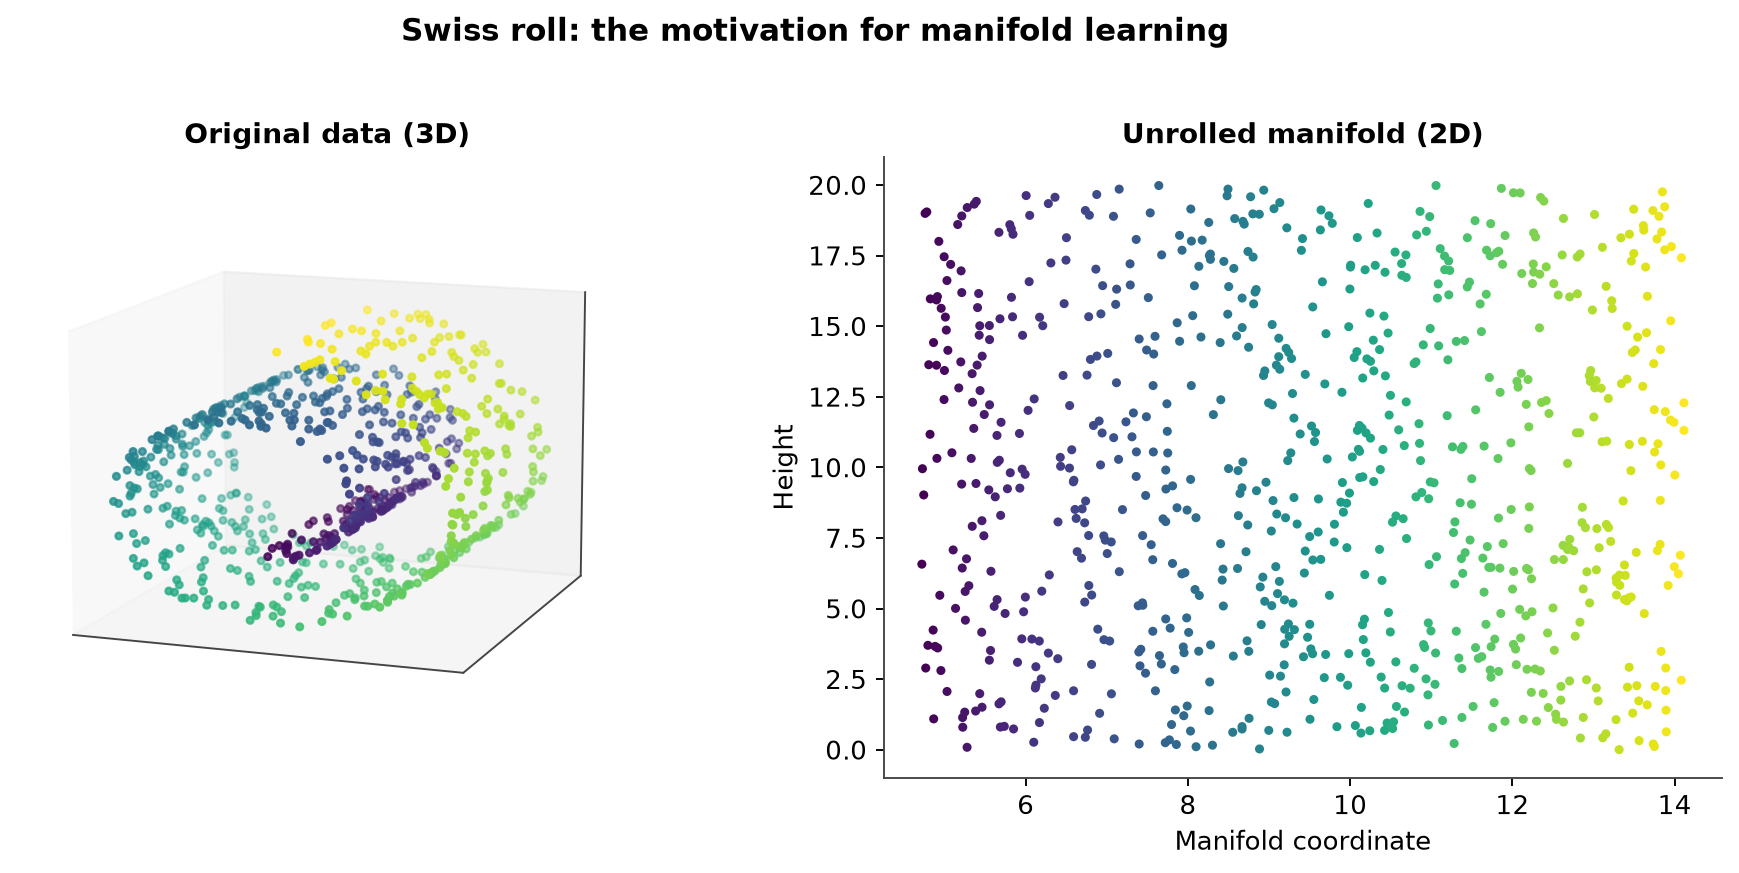
\includegraphics[width=0.7\textwidth]{../book/_static/generated/figures/en/swiss_roll_manifold.png}
  \end{center}
\end{frame}

\begin{frame}{Kernel PCA: the kernel trick}
  \begin{itemize}
    \item Maps the data into a higher-dimensional space where it \textit{is} linearly separable
    \item Useful when the original data can't be split by a straight line
  \end{itemize}
  \begin{center}
    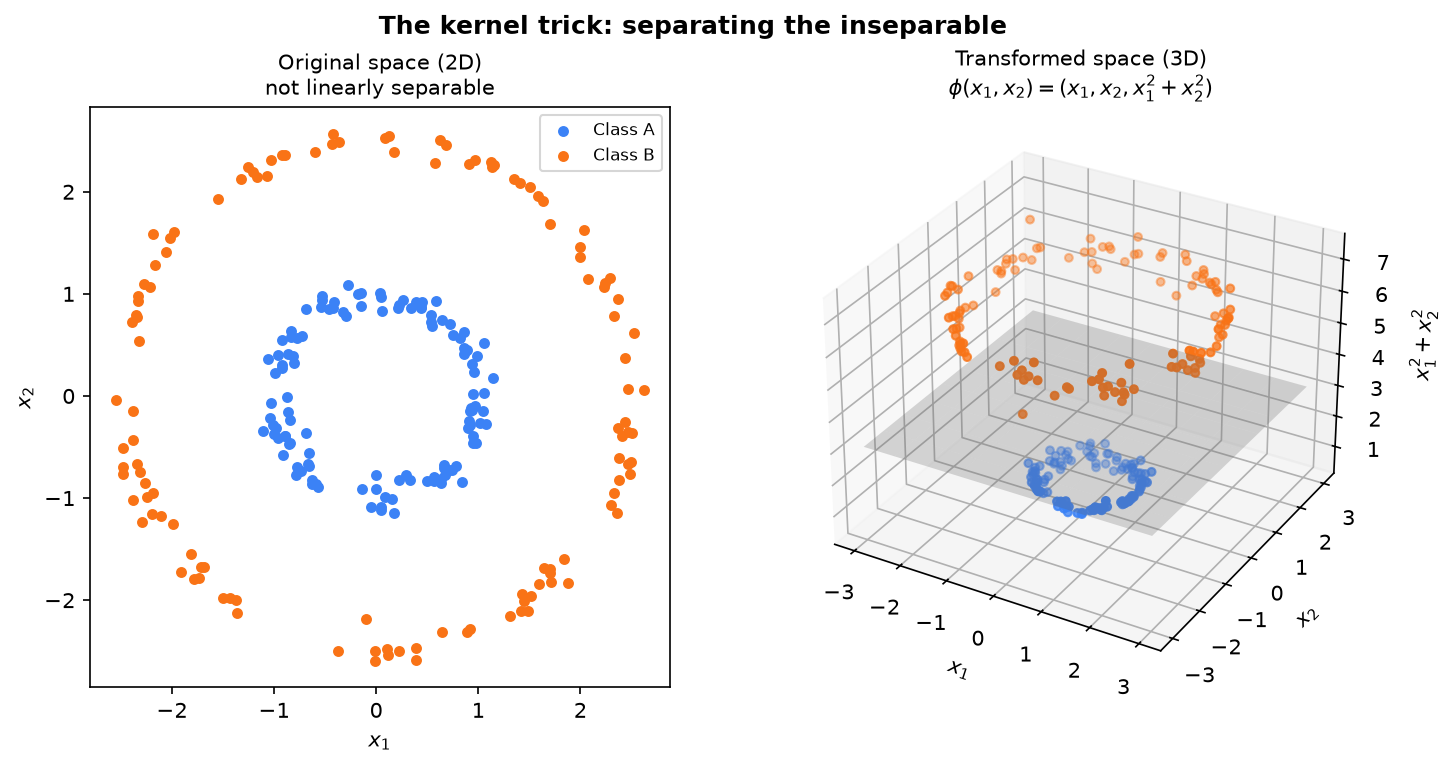
\includegraphics[width=0.72\textwidth]{../book/_static/generated/figures/en/kernel_pca_trick.png}
  \end{center}
\end{frame}

\begin{frame}{t-SNE: preserving local neighborhoods}
  \begin{itemize}
    \item Turns distances into neighborhood probabilities: nearby points should stay close after projection
    \item Excellent for \textbf{visualizing} complex clusters in 2D; slower on large datasets
  \end{itemize}
  \begin{center}
    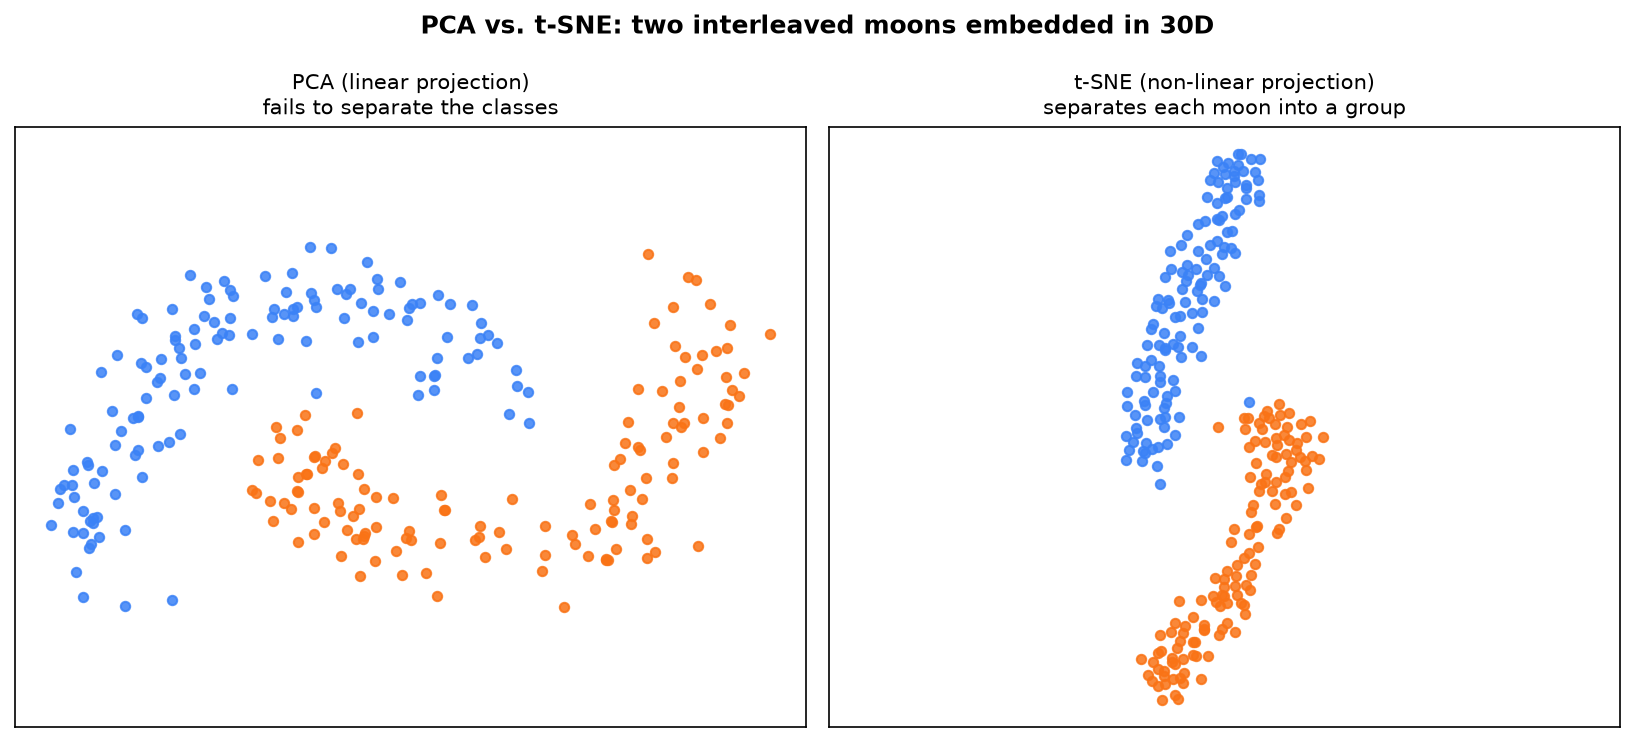
\includegraphics[width=0.78\textwidth]{../book/_static/generated/figures/en/pca_vs_tsne.png}
  \end{center}
\end{frame}

\begin{frame}{UMAP: fast and accurate}
  \begin{itemize}
    \item Preserves both \textbf{local} and \textbf{global} structure, unlike t-SNE
    \item Much faster: suitable for datasets with millions of samples
  \end{itemize}
  \begin{center}
    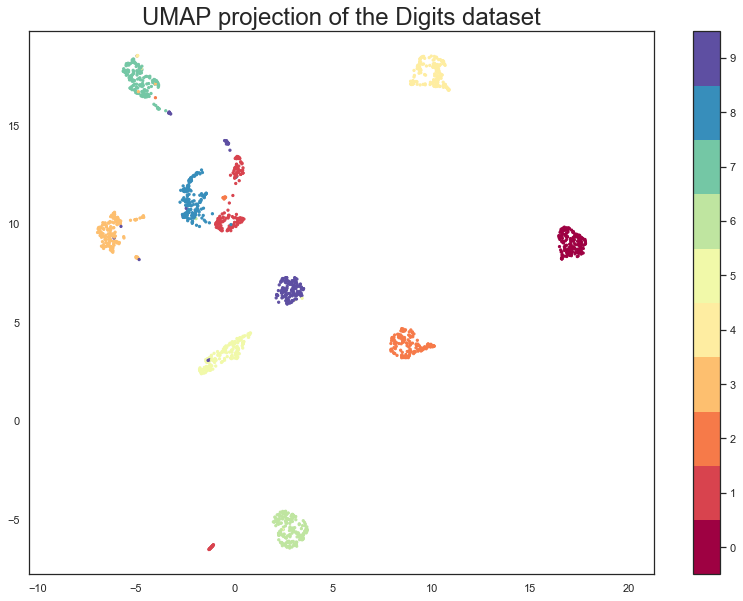
\includegraphics[width=0.4\textwidth]{../book/_static/external_images/umap_digits_projection.png}
  \end{center}
  \fuente{umap-learn docs, Copyright (c) 2017 Leland McInnes, BSD-3 license.}
\end{frame}

\begin{frame}{Summary: 3.2 Dimensionality reduction}
  \begin{itemize}
    \item \textbf{PCA}: fast, linear, interpretable
    \item \textbf{Kernel PCA}: extends PCA to non-linear structures
    \item \textbf{t-SNE}: excellent visualization, non-linear, slow on large data
    \item \textbf{UMAP}: the best balance of speed and quality
  \end{itemize}
\end{frame}

% ============================================================
\section{3.3 Anomaly detection}

\begin{frame}{Philosophy of anomaly detection}
  \begin{itemize}
    \item \textit{Inliers} (normal): frequent, with consistent patterns
    \item \textit{Outliers} (anomalies): rare, deviate significantly from the norm
    \item \textbf{Anomaly detection}: training data may contain noise
    \item \textbf{Novelty detection}: training data is completely clean
  \end{itemize}
  \ejemplo{bank fraud, failures on a production line, or a sensor giving strange readings: in none of these cases do we know in advance what the next anomaly will look like.}
\end{frame}

\begin{frame}{Gaussian approach}
  \begin{itemize}
    \item A Gaussian distribution is fit to the normal data
    \item Points with \textbf{low probability density} are flagged as anomalies
    \item The threshold can be set from the known historical rate of rare cases
  \end{itemize}
  \begin{center}
    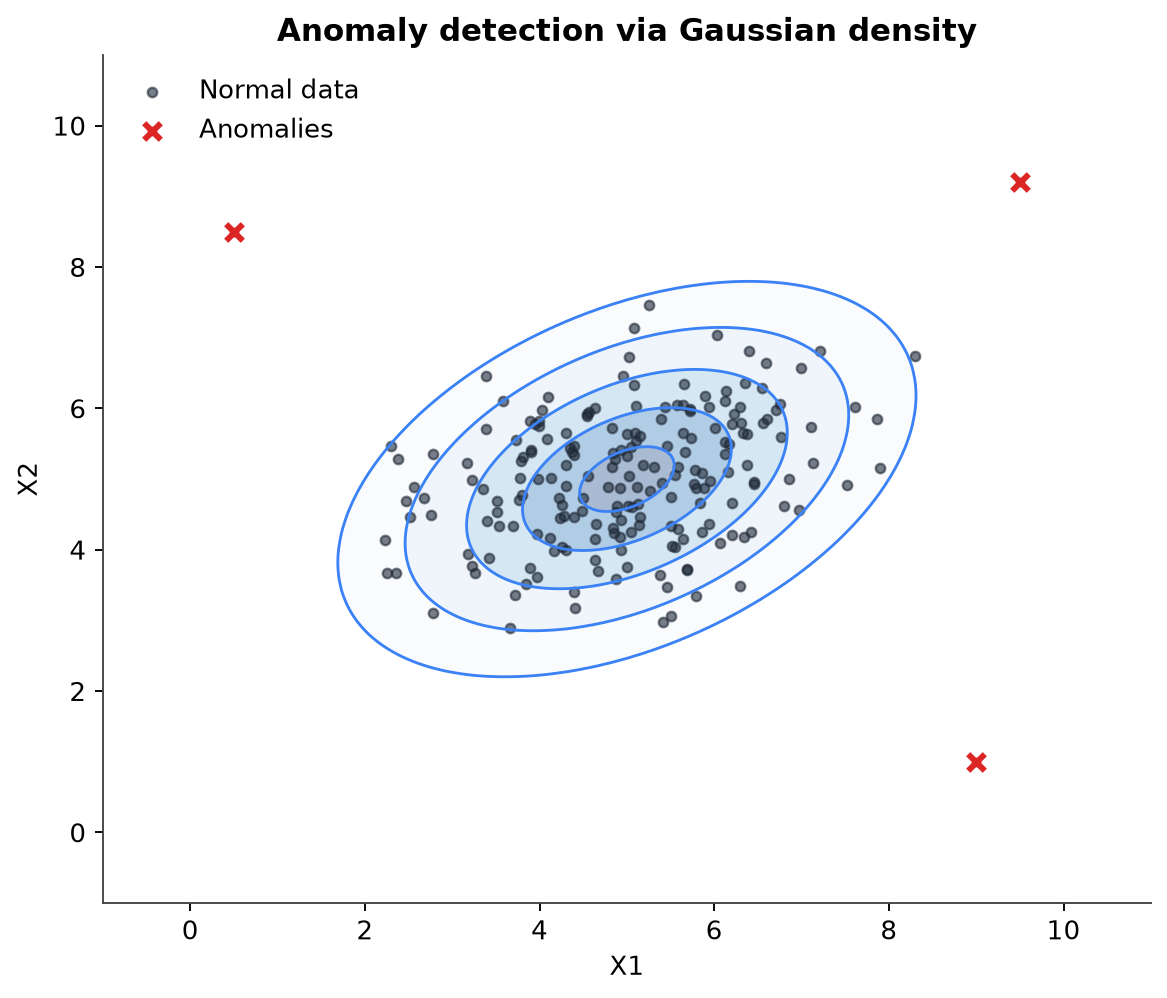
\includegraphics[width=0.4\textwidth]{../book/_static/generated/figures/en/gaussian_anomaly_detection.png}
  \end{center}
\end{frame}

\begin{frame}{PCA reconstruction}
  \begin{itemize}
    \item Data is projected to a low dimension with PCA and then reconstructed back
    \item Anomalies don't follow the main structure, so their \textbf{reconstruction error} is much larger
  \end{itemize}
  \begin{center}
    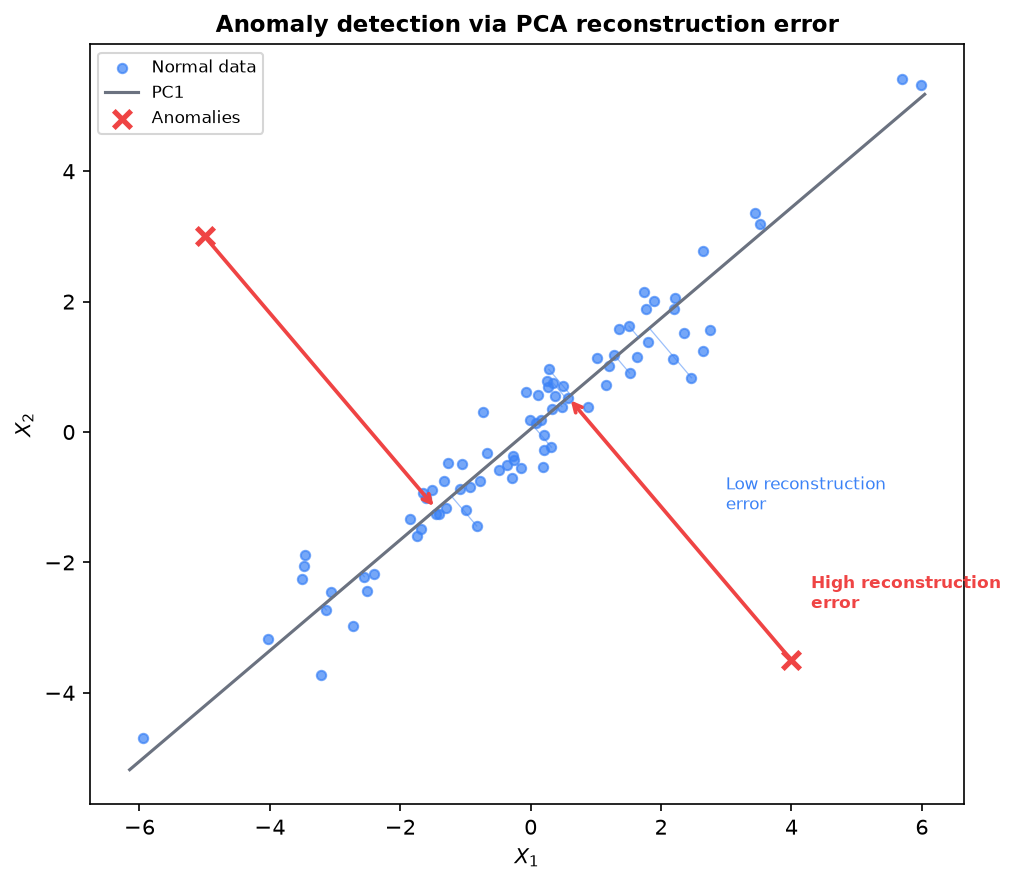
\includegraphics[width=0.36\textwidth]{../book/_static/generated/figures/en/pca_reconstruction_anomaly.png}
  \end{center}
\end{frame}

\begin{frame}{Isolation Forest}
  \begin{itemize}
    \item Instead of modeling what's normal, it tries to \textbf{isolate} each point using random partitions
    \item Anomalies, being far from the rest, get isolated with very few partitions
  \end{itemize}
  \begin{center}
    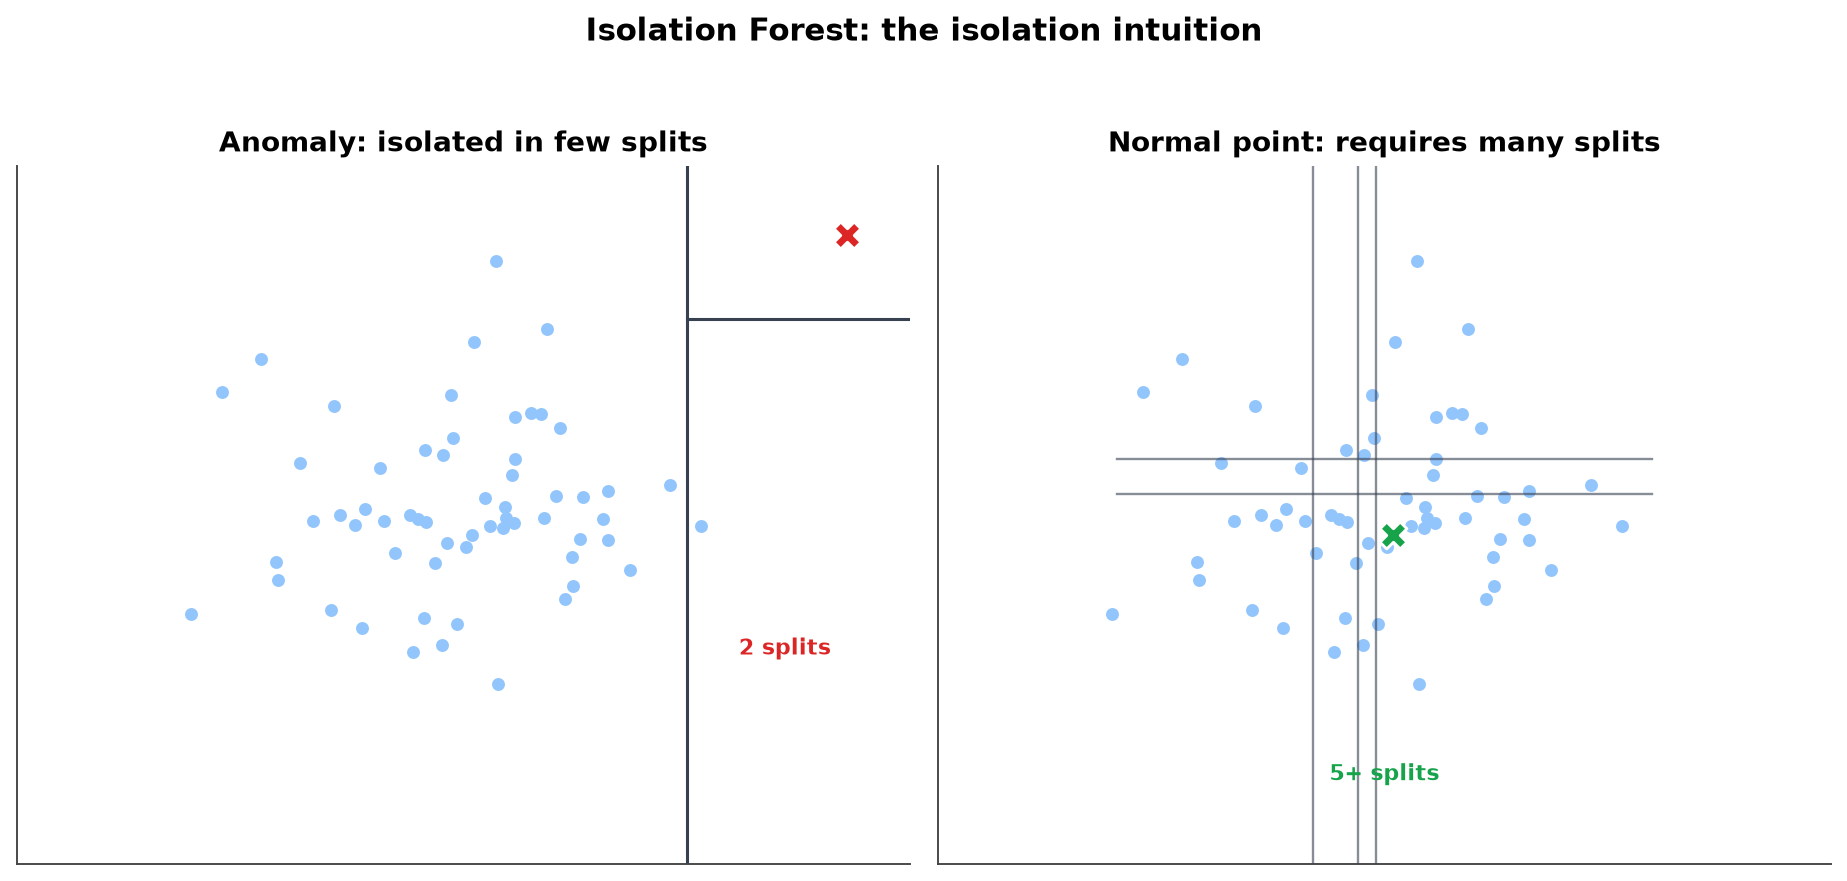
\includegraphics[width=0.85\textwidth]{../book/_static/generated/figures/en/isolation_forest_concept.png}
  \end{center}
\end{frame}

\begin{frame}{Local Outlier Factor (LOF)}
  \begin{itemize}
    \item Compares a point's \textbf{local density} with that of its neighbors
    \item Detects \textbf{local anomalies}: points that aren't extreme in absolute terms, but are unusual in their neighborhood
  \end{itemize}
  \ejemplo{a 200 m\textsuperscript{2} house isn't unusual nationwide, but it is in a neighborhood where every house is 60 m\textsuperscript{2}: that's exactly what LOF detects.}
  \begin{center}
    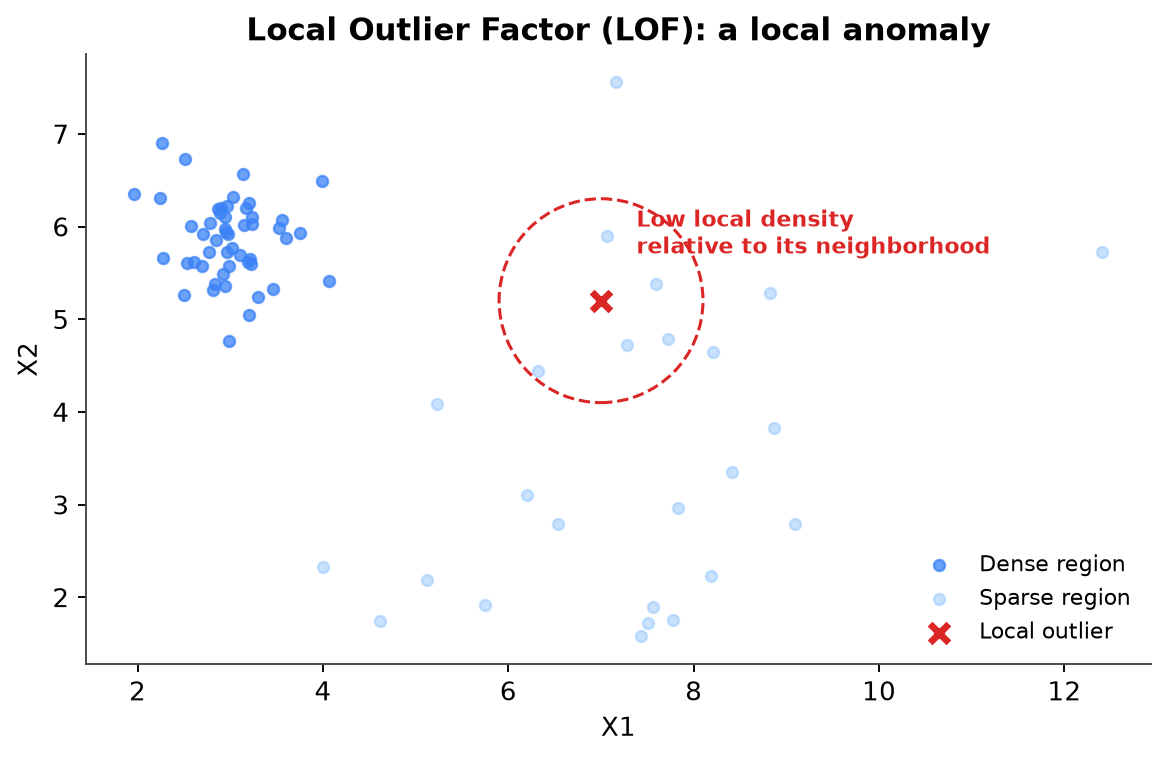
\includegraphics[width=0.32\textwidth]{../book/_static/generated/figures/en/lof_concept.png}
  \end{center}
\end{frame}

\begin{frame}{One-class SVM}
  \begin{itemize}
    \item Designed for novelty detection: trained on clean data
    \item Finds the \textbf{minimum-volume} region that encloses nearly all the training data
    \item Any new observation falling outside that boundary is flagged as an anomaly
  \end{itemize}
  \begin{center}
    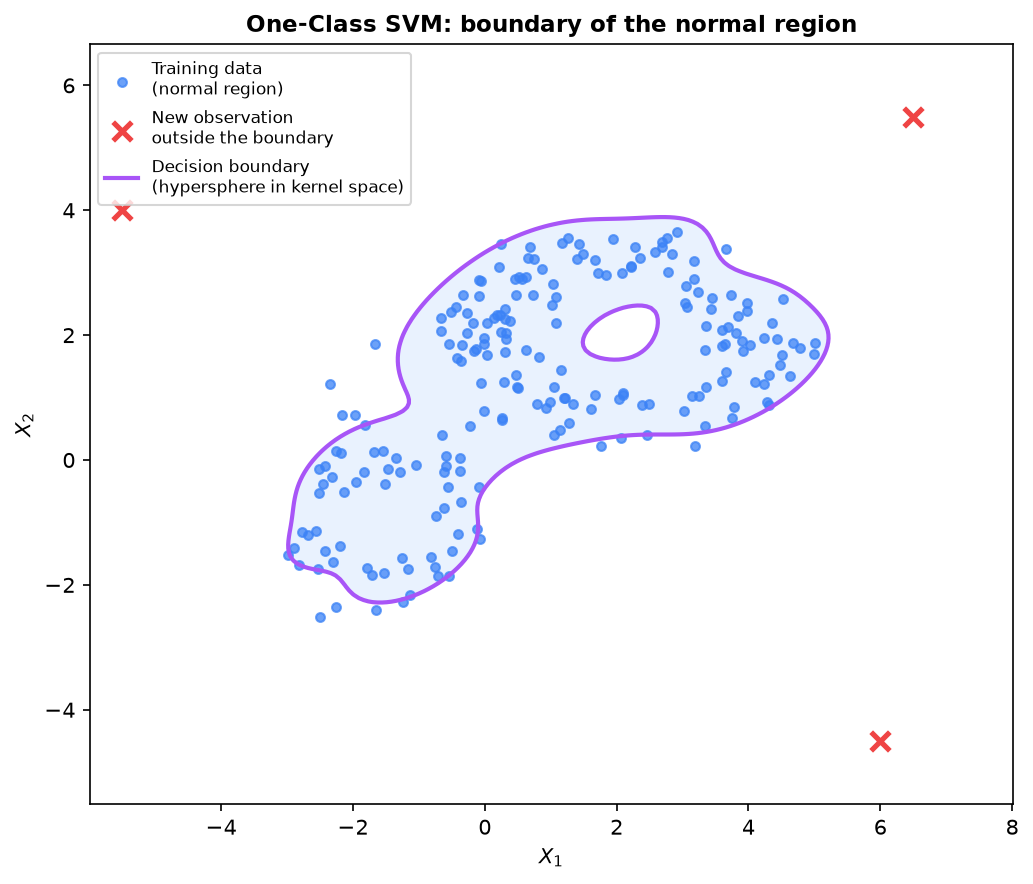
\includegraphics[width=0.36\textwidth]{../book/_static/generated/figures/en/one_class_svm_boundary.png}
  \end{center}
\end{frame}

\begin{frame}{Summary: 3.3 Anomaly detection}
  \begin{itemize}
    \item Anomalies can be rare, contextual, or collective events
    \item \textbf{Simple methods}: Gaussian, PCA reconstruction
    \item \textbf{Advanced methods}: Isolation Forest, LOF, one-class SVM
  \end{itemize}
\end{frame}

% ============================================================
\begin{frame}{Course summary}
  \begin{columns}
    \begin{column}{0.33\textwidth}
      \textbf{1. Foundations}
      \begin{itemize}
        \footnotesize
        \item History of ML
        \item Overfitting/underfitting
        \item Cross-validation
      \end{itemize}
    \end{column}
    \begin{column}{0.33\textwidth}
      \textbf{2. Supervised}
      \begin{itemize}
        \footnotesize
        \item Regression, regularization
        \item Classification, SVM
        \item Neural networks
      \end{itemize}
    \end{column}
    \begin{column}{0.33\textwidth}
      \textbf{3. Unsupervised}
      \begin{itemize}
        \footnotesize
        \item Clustering
        \item PCA, manifold learning
        \item Anomaly detection
      \end{itemize}
    \end{column}
  \end{columns}
\end{frame}

\begin{frame}
  \centering
  {\Huge Thank you!}\\[1em]
  {\large Universidad de Salamanca}
\end{frame}

\end{document}
